%!Tex root=../report.tex

\section{Background}


\subsection{Monte Carlo Tree Search}

Monte Carlo Tree Search (MCTS) is a heuristic algorithm that is used for online planning. It is easiest explained in relation to games. Take for example a game of chess. The goal is to capture the opponents king while keeping your own king safe. However, in order to obtain that goal a number of moves have to be made by you and your opponent alternatively. Deciding which move to make, given the state of the game, is key to winning the game. Moves can have direct rewards (like the capture of an opponents piece), but in general the effect of a move is only noticed a few turns after it has been made (for example when sacrificing a piece or gaining positional advantages). For this reason it is hard to estimate how good a move is without thinking a few steps ahead. Thinking ahead is, however, considerably hard, given the number of options a player has each turn. At the start of the game, a player can make 20 different moves (sixteen with pawns, four with knights), likewise his opponent also has 20 different moves, resulting in 400 possibilities in the first two moves alone. Without proper knowledge of the values of moves, it is hard to judge which would be the best to play. At the same time, it is infeasible to check all possibilities. 

MCTS solves this problem by only evaluating a selected number of combinations and selecting the move with the highest expected reward. For this purpose MCTS constructs a tree that models the game. In this tree, the root is the starting state, the children are the resulting states of a move and the leafs represent the end state of a game. Each node has a value attached to it, which refers to the expected reward. The tree is constructed by sampling different combinations of actions (paths through the tree). When the leaf node is reached, a reward is obtained which is then propagated back to the root. Every node can update its own expected reward with the obtained value by averaging it over all the obtained rewards. Each tree traversal is called a simulation. In order to make sure the MCTS does not take forever, the amount of simulations is limited. In games where it might take a lot of time to reach an end state, a horizon is added to limit the depth of the traversal.  

\subsection{Partially Observable Monte-Carlo Planning}
In many practical problems, the true state of the entire world is not known; instead, a belief may exist regarding the state of other elements, which can be updated with each new observation. Planning problems in which the environment is only partially observable are called POMDPs. These environments pose a challenge for search algorithms; at each point in time an action must be selected of which the long-term consequences are ever less certain. Silver \& Veness observe that Monte-Carlo search trees are well-suited to deal with this uncertainty and propose to extend MCST algorithms with a belief-state filter to apply these to POMDPs (naming the new algorithm POMCP) \cite{silver2010monte}. The motivation is that the Monte-Carlo process effectively simulates probability distributions of rewards, removing the problem of explicitly factorizing the true distributions. Indeed, Silver \& Veness find that MCTS yields superior performance to previous approaches on three games with various state-space sizes and dynamics. The POMCP algorithm, with a description of its process, is illustrated in \ref{fig:pomcp} (originally from \cite{silver2010monte}). 

\begin{figure*}[ht!]
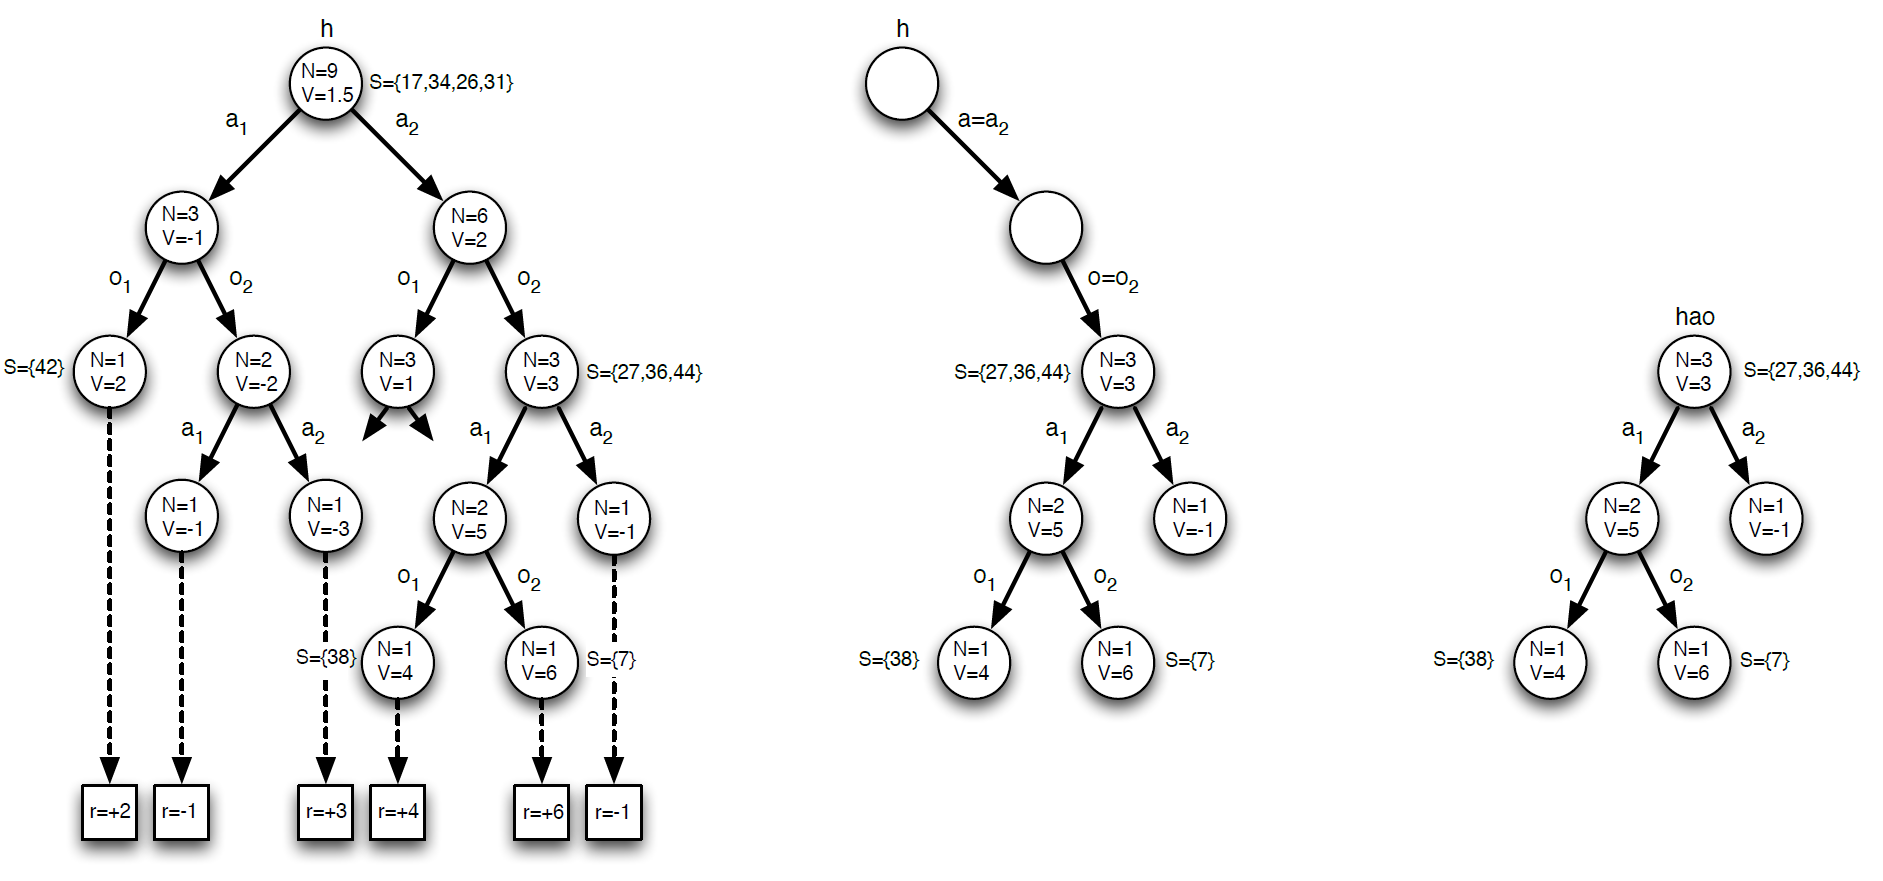
\includegraphics[width=\linewidth]{pomdp.png}
\label{fig:pomcp}
\caption{An illustration of the three steps in a single step of the POMCP process, from \cite{silver2010monte}. Each step in the tree consists of an action and corresponding observation. The algorithm first simulates a large number of actions and potential observations (left), then aggregates the rewards and chooses the action with the highest mean return (middle) to which it receives the true observation. Finally, the believe-state is updated and the tree is pruned, the process starts again with the new state (right).}
\end{figure*}
